
\chapter[Renderización de la geometría de Panes]{Renderización de la geometría de Panes y otros Materiales Porosos}
\section{Introducción}
Debido a las limitaciones existentes actualmente en el renderizado realista de pan, nos proponemos en este capítulo estudiar la utilización de renderizado directo de volúmenes aplicado a un campo escalar representando la geometría de la miga de pan. 

%Los resultados obtenidos son realistas y se renderizan en tiempo real. La misma evita el uso de estructuras intermedias, simplificando el desarrollo y reduciendo los costos computacionales.
El renderizado foto-realístico de materiales con una estructura interna compleja presenta grandes retos en Computación Gráfica.
En particular, las migas de panes son un material translúcido complejo, con una estructura porosa, que presenta detalles diferentes en distintas escalas, todos igualmente necesarios de ser tenidos en cuenta para lograr una correcta visualización.
El renderizado realista de estos materiales debe simular correctamente diversos fenómenos como translucencia, auto-sombreado, auto-oclusión, reflectancia, y absorción, entre otros.

Las técnicas del estado del arte en renderizado de migas de panes tratan el material como una superficie, seteando un complejo procedimiento de captura, en el cual la luz reflejada por el material es fotografiada en distintos ángulos.
Luego, la información es procesada y reconstruída para formar un modelo del material.
Si bien esta solución es capaz de capturar los fenómenos lumínicos previamente discutidos, también es cierto que la practicidad del método está severamente comprometida, ya que presenta un costo computacional alto, un procedimiento de captura muy limitado y la imposibilidad de obtener más de una apariencia con una única captura.

En un intento por superar estas limitaciones del renderizado, proponemos, en conjunción con el capítulo anterior de modelado de la geometría, utilizar un modelo volumétrico del pan.
Para esto utilizamos la técnica de renderizado directo de volúmenes, implementada en GPU.
La técnica permite renderizar los campos escalares del capítulo anterior sin utilizar estructuras intermedias.
Las imágenes obtenidas son promisorias, y se computan en tiempo real gracias al poder de las placas gráficas actuales.

\section{Trabajo Previo}
El tópico de renderizado foto-realista de materiales, y su modelado, atrajo un interés creciente en la literatura científica.
La mayoría de los esfuerzos están focalizados en materiales complejos de frecuente aparición como el agua \cite{Schechter2012}, la piel humana \cite{Donner2006}, metales, plásticos \cite{Kurt2010}, etc.
La comunidad de investigadores, sin embargo, ha tenido grandes dificultades para simular adecuadamente la apariencia de otros materiales, como es el caso de materiales cocidos ({\em e.g.}, pizza, galletitas).
Debido a su compleja geometría y fenómenos lumínicos involucrados, esto continúa siendo un problema abierto \cite{Voglsam2013}.

Hasta hace pocos años, el costo computacional de renderizar modelos físicos de estos materiales resultaba prohibitivo si el tiempo real era un requerimiento.
De todas formas, el crecimiento notable en poder de cómputo debido al diseño masivamente paralelo de las placas gráficas \cite{Yeo09,Harris06}, está permitiendo la simulación de complejos fenómenos de interacción de la luz con los materiales en tiempos de cómputo aceptables.

Simulating an acceptable bread geometrical model represents an additional challenge.
This and other kinds of porous structures are the result of complex mechanisms involving physical deformations, heat and mass transport during baking, and several chemical reactions.

Recent studies employs phenomenological considerations on real breads, but the geometry is fixed ({\em i.e.}, non procedural) \cite{VanDyck2014}: a fixed geometry does not allow to obtain several different bread types easily, since it requires a capture procedure for each of them, and, in addition, bubble distributions can be neither controlled nor changed.

%Different rendering algorithms are targeted to different data structures. Particularly, triangular meshes should be derived from voxel data (marching cubes \cite{Lorensen1987}). Nevertheless, the construction of a porous bread structure can demand large amounts of memory.

The presence of mesostructures (bubbles and alveoli of complex shapes) makes bread a quasi homogeneous material \cite{Tong2005}. 
For this reason, adequate surface representations of this material are not possible.
Typical techniques such as Bidirectional Reflectance Distribution Functions (BRDFs)
\cite{Kurt2009}, and Bidirectional Surface Scattering Reflectance Distribution Functions (BSSRDFs) \cite{Donner2009}, are not satisfactory.
A material model \cite{Tong2005} solves these limitations, but the associated drawbacks (complex capture procedure involved, computational costs, poor geometry variability),
makes the method far from practical.

On the other hand, research on physically inspired mathematical models of bread crumbs is not uncommon in the food industry related literature.
These works aim to adequately model and simulate heat and mass transfer in dough during baking, among other issues.
Recent results suggest that 1D models could suffice, for instance modeling the geometry as an infinite cylinder, or assuming only one radial coordinate \cite{Purlis2012, Thorvaldsson1999}.
These and other results in the food industry have some significance in bread crumb modeling and rendering, and may be used as a further basis for computational baking models. 


\section{Renderizado Directo de Volúmenes (DVR)}
The technique of Direct Volume Rendering (DVR)\cite{Kratz2006} generates two-dimensional images by computing the interaction of light with a semi-transparent medium that is represented by a discrete scalar field.
This field describes the density of the medium at regular sample points. 
For each pixel in the image a ray is cast from the camera position and the radiance reaching the camera from its direction is computed by approximating the radiative transfer equation (RTE). This equation describes the change in radiance along a ray as it traverses non-transparent media.
In its complete form, the RTE incorporates many different optical properties and effects. 
In order to approximate the result of the RTE in real-time, this work uses a simplified version of the equation that only incorporates some of the optical phenomena that occur in reality.

There are three important optical phenomena that affect the propagation of light through a medium at a given point in space: emission, absorption and scattering.
Emission is the generation of radiant energy in a given direction.
Absorption happens when a fraction or all of the radiant energy in the light ray hits an opaque object and is transformed into other forms of energy. 
%
Finally, scattering events result in the change of direction of photons. 
Scattering events that cause photons to change directions away from the direction of a ray are called out-scattering events. Conversely, in-scattering events result in photons changing direction towards the ray direction.
%
The contribution of in-scattering is often computed for radiance from a single direction which corresponds to the main light source of the scene.
This corresponds to the radiative energy arriving at a point from the light source, bouncing on the particles in the medium at that point and then traveling along a given ray direction.

The RTE can be summarized as:

\begin{equation} \label{eq:general_radiance}  
  L(p_n) = L_b + \int_{p_0}^{p_n} \frac{\partial L(t)}{\partial p} \, dt,
\end{equation}

\noindent where $L_b$ is the background radiance, and $p_0$, $p_n$ are the closest and furthest visible points along the ray direction, respectively, $L(t)$ is the radiance at point $t$, and $\partial p$ is the distance between sampled points. 
Since the input to the DVR algorithm is a discrete data set, in order to compute $L(p_n)$ the integral is approximated by a sum.

Extinction is the decrease in radiance in a ray due to absorption and out-scattering.
We can approximate this effect by defining an absorption coefficient for the media, $k_a$ and an out-scattering coefficient $k_s$. 
If we neglect the out-scattering effect, the formula that describes the radiance reaching a point after traversing a ray segment is:

\begin{equation} \label{eq:radiance_absorption}  
    L_b \ e^{- \textstyle  \int_{p_0}^{p_n} k_a(t) \, dt}.
\end{equation}

We introduce the value $\int_{p_i}^{p_j} k_a(t) \, dt$, the absorption coefficient, and we will refer to it as $\tau_{(p_i, p_j)}$. 
Transmittance is complementary to extinction. It describes the amount of light passing through a medium in a given direction. 
The transmittance value along two points $p_i$ and $p_j$ is thus:

\begin{equation} \label{eq:transmittance}  
  T(p_i,p_j) = e^{- \textstyle \tau_{(p_i, p_j)}}.
\end{equation}

If we assume that at every point inside the volume along the ray there is an increase of radiance due to emission and in-scattering phenomena ($\rho$), then our initial radiance estimate becomes:

\begin{equation} \label{eq:ray_radiance}  
  L(p_n) = L_b \ e^{-\tau(p_0, p_n)} + \int_{p_0}^{p_n} \rho \ e^{-\tau(t,p_n)} \, dt.
\end{equation}


This means that the radiance along points $p_0$ and $p_n$ is the attenuated remaining background radiance plus the attenuated emission and in-scattering at every ray point.
The DVR algorithm samples the volume density function at regular intervals, approximates the transmittance along those points and computes the amount of light reaching the camera along the ray direction.
The computation replaces the integral sum by a discrete sum over the length of the ray intersecting the volume:

\begin{equation} \label{eq:ray_radiance}  
  L(p_n) = L_b \ e^{-\tau(p_0, p_n)} + \sum_{p_0}^{p_n} \rho \ e^{-\tau(p_i,p_n)}.
\end{equation}

Other effects can be accounted for, augmenting the final image's fidelity, as well as the technique's computing cost. 
The basis of our rendering algorithm uses the simplified transmittance and emission only model, along with some artistic considerations, to achieve real time frame rates.
The rendering algorithm is described in detail in a further section. 
%~\ref{sec:rendering}.
%%%%%%%%%%%%%%%%%%%%%%%%%%%%
%La técnica de DVR tiene como objetivo crear una representación bidimensional de un volumen
%definido por una función de densidad tridimensiopocnal. Para ello, se emiten rayos desde el punto de vista de una cámara en una escena virtual y se utiliza la función de densidad para calcular la cantidad de luz que la cámara recibe en la dirección del rayo. Para esto se evalúa la función de densidad en el camino del rayo y se usan los valores adquiridos para aproximar el efecto de varios fenómenos lumínicos, como pueden ser la extinción, transmitancia, o dispersión lumínica, entre otros. La información obtenida de procesar todos los rayos se utiliza para definir el color de los pixeles en la imagen final.

%La radiancia es la cantidad de luz que pasa, o es emitida, desde un punto y atraviesa un determinado ángulo sólido. En el contexto de DVR, el medio que los rayos atraviesan, y que es definido por una función de densidad, es considerado como emisivo. Por lo tanto, cuando se busca calcular la cantidad de luz recibida en la dirección de un rayo, lo que se hace es aproximar la radiancia recibida de un punto distante siguiendo la dirección del rayo. El valor de la radiancia es aproximado como la suma de una radiancia de fondo y la radiancia emitida por el medio por el cuál se mueve el rayo \cite{Kratz2006} :

%\begin{equation} \label{eq:general_radiance}  
%  L(p_n) = L_b + \int_{p_0}^{p_n} \frac{\partial L(t)}{\partial p} \, dt,
%\end{equation}

%\noindent donde $L_b$ es la radiancia de fondo, $p_0$ y $p_n$ son los puntos inspeccionados en la dirección del rayo más cercano y más lejano respectivamente, $L(t)$ es la radiancia evaluada en el punto $t$, y $\partial p$ es la distancia entre puntos evaluados. En el momento de calcular $L(p_n)$, la integral es aproximada por una suma.

%La extinción es la pérdida de fotones en un haz de luz debido a la absorción en el medio que atraviesa y la dispersión hacia otras direcciones. Algunos de los fotones colisionarán con particulas del medio y serán absorbidas y transformadas en otras formas de energía, mayormente calor. Otras rebotarán y pasarán a moverse en otras direcciones. Estos fenómenos se aproximan usando un coeficiente de absorción para el medio, $k_a$ y un coeficiente de dispersión $k_s$. Si el efecto de dispersión es ignorado, la fórmula que define la cantidad de radiancia absorbida en el largo de un segmento de rayo
es: 

%\begin{equation} \label{eq:radiance_absorption}  
%    L_b \ e^{- \textstyle  \int_{p_0}^{p_n} k_a(t) \, dt}.
%\end{equation}

%El valor $\int_{p_i}^{p_j} k_a(t) \, dt$ es llamado coeficiente de absorción y se referenciar\'a como $\tau_{(p_i, p_j)}$.

%La transmitancia es un concepto complementario a la extinción y describe la cantidad de luz que pasa por un medio en una dirección determinada. El valor de transmitancia entre dos puntos $p_i$ y $p_j$
%es:

%\begin{equation} \label{eq:general_radiance}  
%  T(p_i,p_j) = e^{- \textstyle \tau_{(p_i, p_j)}}.
%\end{equation}

%Si la emisión de luz se asume como un término constante ($\rho$) para todos los puntos del medio, la fórmula inicial de radiancia queda:

%\begin{equation} \label{eq:ray_radiance}  
%  L(p_n) = L_b \ e^{-\tau(p_0, p_n)} + \int_{p_0}^{p_n} \rho \ e^{-\tau(t,p_n)} \, dt.
%\end{equation}

%Esto significa que la radiancia entre los puntos $p_0$ y $p_n$ se puede calcular como la radiancia de fondo restante luego de la atenuación del medio sumada a la emisión, también atenuada, en todos los puntos del medio que atraviesa el rayo.

%La técnica de DVR define un volumen donde una función de densidad se evalúa en intervalos regulares y utiliza esa información para aproximar la transmitancia en esos puntos y de esa manera aproximar la cantidad de luz que llega a la cámara. La suma integral descrita anteriormente se reemplaza por una suma discreta de los puntos evaluados de un rayo donde \'este intersecta al volumen que interesa representar. 

%Otros efectos lumínicos pueden ser aproximados. Esto aumenta la fidelidad de la imagen final pero también aumenta el costo de cómputo de la técnica. Algunos de estos efectos son el cálculo de fase, el c\'alculo de luz entrante por dispersión o luz extinguida por dispersión, entre otros. Dado que el objetivo de este trabajo es lograr un renderizado en tiempo real, el algoritmo implementado usa como base el modelo de cálculo de radiancia simplificado que toma en cuenta sólo la
%transmitancia del medio.

\section{Implementación}


We created a demo application \footnote{available at \emph{https://www.github.com/rbaravalle/Pysys}} that uses the particle system described in the previous sections to render real-time bread models using a DVR approach. 
In this demo we produced a volume texture from the original particle system.
A cube that corresponds to this volume is then rendered in the scene.
The material used to render the cube uses a very simple vertex shader and a fragment shader that implements the DVR algorithm. For each fragment, this shader computes a ray originating from the camera position and in the direction of the fragment that must be shaded. 
The procedure samples the volume texture at regular intervals along the intersection of this ray and the cube.
The sample values are then used as input of a simplified version of the radiative transfer equation to compute the resulting pixel color as described in previous sections.
%~\ref{sec:DVR}.
We employ these equations to accumulate the transmittance of the ray and the radiance contribution at every sample point.
The computation ends if the transmittance falls below a threshold value or if the ray exits the cube. 
Single in-scattering is approximated by computing a secondary ray at each sample point directed towards the scene light source.
This secondary ray is then sampled to determine the amount of light that reaches the original sample point. 
This technique allows to naturally perform self shadowing within the model.

We shade the pixel using the primary and secondary ray transmittance information. 
At this point, different artistic considerations may be applied to yield different
looking materials.
For instance, we can differentiate crumb and crust by assigning a higher extinction coefficient and a darker color to crust regions. 
A soft yellowish color applied in other regions provides a crumb appearance.
Additionally, it is possible to add a faint specular reflection. 
The contribution of that reflection is computed at the first intersection point between the ray and the particle system in order to increase the final image realism. 
The normal vector used for this computation is the gradient of the volume texture at that point.

The demo we present provides the user with the ability to modify parameters such as the transmittance coefficient, the transmittance threshold, the color assigned to the crumb and the visibility of the specular highlights. 
By modifying these parameters the user can produce images that resemble other porous materials, such as sponges.

\subsection*{Ambient Occlusion}

One key aspect to enhance the final image appearance is the local contributions due to tiny material features (emission, occlusion, absorption). 
Previous works show that considering ambient occlusion can greatly enhance synthetic image realism \cite{Hernell2010}.
Based on this idea we approximate multiple in-scattering by computing (offline) an ambient occlusion term for each voxel in the scalar field and storing it as an additional volume texture, which is used by the fragment shader.

For each voxel, the algorithm sets a neighborhood of radius $r$ and stores the mean voxel value within that radius in the ambient occlusion texture.
It then uses this value to modulate the contribution of a ray sample.
Setting different values for $r$ produces similar results. 
Fig.~\ref{fg:occlusion} shows that the enhancement added using ambient occlusion clearly improves the final image appearance and is a key aspect in realistic bread appearance. It is worth mentioning that the net effect of this term was somehow oblivious to the radius $r$ of the surrounding sphere, for $r > 0$.
 
\subsection*{Normals Computation}

We use a simple forward difference schema for the gradient computation. In this method, we compute the normal vector at a point using the gradient, represented as the normalized difference vector between the field values at the forward positions and the actual position:

\begin{equation}
\begin{aligned}
x &= tex(pos+(1,0,0)) - tex(pos)\\
y &= tex(pos+(0,1,0)) - tex(pos)\\
z &= tex(pos+(0,0,1)) - tex(pos) \\
N &= normalize([x,y,z])
\end{aligned}
\end{equation}

We use the normals and the light vector to determine the specular contribution, applying a simple Phong model \cite{Phong1973}, with a parameter that lets the user change the impact of the specular component.
We tested other more accurate specular models, but there was no appreciable difference in the final bread appearance.

\subsection*{Shadows Computation}

The DVR technique can also be used to compute realistic shadows using shadow maps \cite{Williams1978}.
During the shadow map generation we again render a cube representing the particle system.
The fragment shader for that box uses the same ray-casting method explained above, but only computes the transmittance along the ray. 
If the transmittance along the ray is above a threshold value, then the fragment does not correspond to an occluder and its depth is set at infinity. 
If during the volume traversal the transmittance falls below the threshold, the fragment depth is set to that sample point depth.
This technique is used along with percentage-closer filtering to generate realistic looking shadows in our demo application.

\subsection*{Crust}
We can provide a function that defines whether a volume point is part of the crust or the crumb. For instance, we may provide a function that defines a cylindrical crust envelope by assigning crumb to positions close to the axis of the cylinder, and crust to all other positions. Another function is provided to define whether a point should be considered empty air.
This allows an easy way to define bread crust and slices (see Figs.~\ref{fg:crumb} and \ref{fg:results2}).

\paragraph{Crust determination using Mathematical Morphology}
Since it is difficult or impossible to define mathematical functions that adapt to arbitrary shapes, we propose an automatic method for crust determination using mathematical morphology \cite{Gonzalez2001}.
The idea is to obtain an outer region of the resulting $3D$ scalar field. 
For this, we use basic techniques known as closing, erosion and dilation.

For the purposes of our work, we will define the operations on $3D$ binary scalar fields.
A structuring element $E$ is defined as a binary scalar field representing a particular shape (cube, sphere, etc.).
Structuring elements are employed to perform morphology operations.

The erosion operation can be employed to reduce the total size of a scalar field.
The erosion of a $3D$ scalar field $A$ using a structuring element $B$ is defined as:

\begin{equation}
A \ominus B = \{z\in \mathbb{Z}^3 | B_{z} \subseteq A\},
\end{equation}

\noindent where $B_{z}$ is the translation of $B$ by the $3D$ vector $z$.

The dilation operation is used to augment the total size of a scalar field following its boundary.
The dilation of a $3D$ scalar field $A$ using a structuring element $E$ is defined as:

\begin{equation}
A  \oplus E = \bigcup_{e\in E} A_e.
\end{equation}

The closing operation is used to fill holes in the scalar field.
The closing of a $3D$ scalar field $B$ using a structuring element $E$ is defined as a dilation followed by an erosion:
\begin{equation}
B \bullet E = (B \oplus E) \ominus E,
\end{equation}
see \cite{Gonzalez2001} for further details.

To obtain the outer region of the $3D$ porous volume, we have to eliminate the holes in the scalar field (bubbles) and then compute a boundary.
To do this, the first step performs a closing $c$ of the scalar field using a cube (structuring element of radius $r$), causing the closing of interior bubbles.
Calling $d$ the dilation of $c$ with an spherical element of radius $r_{2}$ and $e$ the erosion $d$ using a spherical structuring element with a slightly shorter radius ($r_{3}$).
The difference between $d$ and $e$ lies in the boundary of the scalar field, so it could be used as a crust.
To eliminate some possible inaccuracies resulting from previous steps, we successively perform a closing of $d-e$ and a dilation to the result, obtaining the final crust.
Fig.~\ref{fg:crusts} shows examples of scalar fields with crusts added using this technique. The results naturally adapt to any scalar field, even with holes.
Since the result would completely cover the scalar field, the crust can be set to span only a subset of the complete volume, allowing the user to see the bread crumb.

%%%%%%%%%%%%%%%

%Se cre\'o un programa de prueba\footnote{disponible en \emph{\url{https://www.github.com/rbaravalle/Pysys}}} para evaluar el sistema de partículas que describe la estructura del pan. Este programa usa un campo escalar representando la miga de pan para generar una textura volumétrica que se interpreta como una función de densidad. Esta textura precomputada se usa como entrada para un motor gráfico que utiliza la técnica de DVR para generar imágenes del pan representado por el sistema de partículas original. Este programa demuestra que el método de renderizado propuesto es compatible con los motores gráficos basados en técnicas de renderización en tiempo real en GPU. Se obtienen imágenes de un material realístico así como efectos de sombras suaves dentro del volumen. Esto significa que las técnicas usadas para renderizar estos materiales pueden ser integradas en cualquier motor de renderizado que soporte shaders.

%La malla que utiliza el modelo es un cubo que contiene el volumen definido por el sistema que genera la miga del pan. El código del shader de vértices es muy simple, proveyendo sólamente información geométrica al shader de fragmentos. Este último es donde se encuentra la mayor parte de los cálculos a realizar.

%Dentro del shader de fragmentos la primera operaci\'on es calcular la geometría de un rayo cuyo origen es la cámara de la escena y cuya dirección lo lleva hacia el fragmento siendo calculado. Este rayo es recorrido en intervalos regulares, evaluando la textura volumétrica para obtener la densidad del pan en esos puntos. Este valor se utiliza para calcular la transmitancia acumulada desde la cámara hasta el punto evaluado. Una vez que la transmitancia es menor que un valor preestablecido o el rayo sale del cubo que define el volumen, el cómputo termina.

%En cada punto evaluado también se computa la transmitancia dentro del volumen desde el punto hacia la fuente de luz en la escena. Esto se hace emitiendo un rayo desde el punto con dirección a la luz y nuevamente calculando la densidad en varios puntos del rayo. Con esta nueva información se aproxima la cantidad de luz que llega directamente al punto considerado, y permite representar sombras dentro del volumen.

%La información de transmitancia de los puntos evaluados del rayo principal y desde estos puntos hacia la luz se utilizan para calcular el color final del fragmento. A partir de esta información y tomando diferentes consideraciones artísticas pueden lograrse representaciones realísticas de diferentes materiales. En el caso de las imágenes de muestra presentadas en este trabajo el color del fragmento será más oscuro para areas del volumen que se consideran dentro de la corteza del pan y será de un color amarillo claro para la miga. También se usa un componente especular tenue. La información de transmitancia entre los puntos evaluados y la luz ayuda a proveer detalles de la estructura del pan. La Fig~\ref{fg:fragmentshader} muestra un esquema del cálculo del color final del pixel.

\begin{figure*}[htb!]
  \centerline{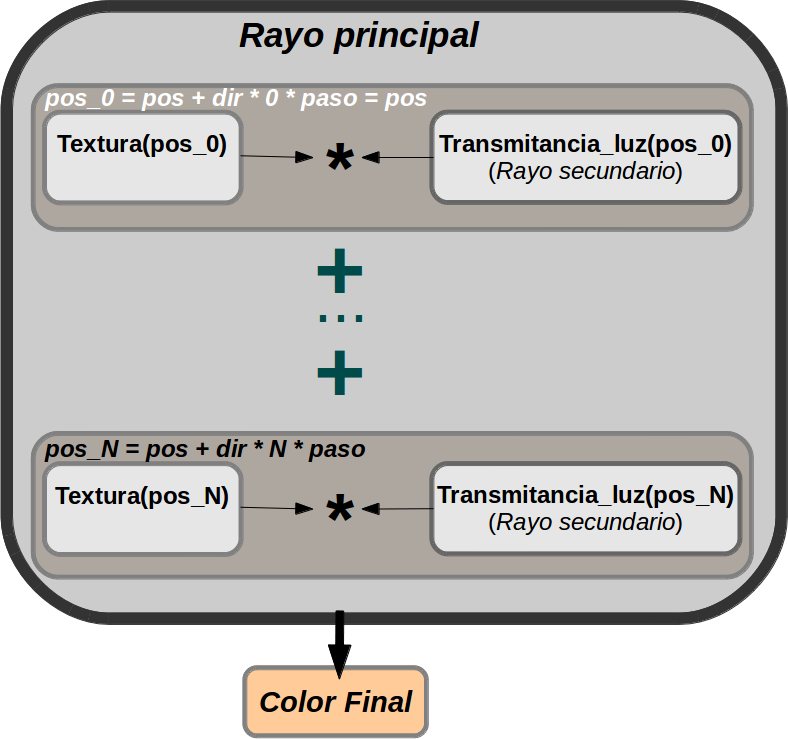
\includegraphics[width=13cm]{fragmentshader}}
  \caption{Cálculo de color en el shader de fragmentos. }
  \label{fg:fragmentshader}
\end{figure*}


El programa de prueba creado permite modificar parámetros tales como el coeficiente de transmitancia del pan, el límite de transmitancia, el color asignado a la miga y la intensidad de los reflejos especulares, entre otros. Esta capacidad permite crear imágenes que semejan otros
materiales porosos, como por ejemplo esponjas.

%\paragraph{Corteza, fetas y cortes}

%Las partes del volumen pertenecientes a la corteza y a la miga del pan fueron determinadas manualmente mediante una función que asigna una u otra propiedad a cada punto del volumen a partir de su posición. Por ejemplo, para volúmenes de forma cilíndrica se definió una función que designa como corteza a los puntos que están a más de una distancia predefinida del eje del cilindro.

%De la misma manera se define una función que determina si puntos del volumen deben considerarse vacíos, independientemente del valor de la textura volumétrica en ese punto. Esto permite definir fetas de pan de manera sencilla. Un ejemplo del uso de este mecanismo puede apreciarse
%en la Fig.~\ref{fg:fig5}.

%La asignación de vacío y de corteza deben ser extendidos más allá de ecuaciones basadas en posiciones para poder ser usadas en un proceso artístico.

%*MORFOLOGIA MATEMATICA*


%En la siguiente sección se presentan y se evalúan los resultados obtenidos.
%
%En esta sección se detallan las imágenes y los tiempos de renderizado obtenidos. 

\subsection{Resultados del renderizado}

%Las imágenes obtenidas a partir del método descrito en la sección anterior fueron renderizadas en una computadora con una placa gráfica nVidia GTX 480 ($480$ cores), la cual es normalmente de uso hogareño. La CPU fue una Intel(R) Core(TM) i5-2300 CPU (cuatro procesadores). La resolución de las imágenes es de $1440\times990$ pixels. 
%Se obtuvieron diferentes imágenes que semejan materiales horneados. Diferentes tipos de pan pueden ser representados variando los parámetros de transmitancia y colores utilizados (ver Fig.~\ref{fg:fig5}). En la imagen central los patrones producidos por los sistemas de partículas descritos en las secciones previas son claramente visibles. En ese caso, el tiempo de vida de las partículas es diferente para cada una y de esa manera se obtienen burbujas de
%diferentes tamaños.

\begin{figure*}[htb!]
  \centerline{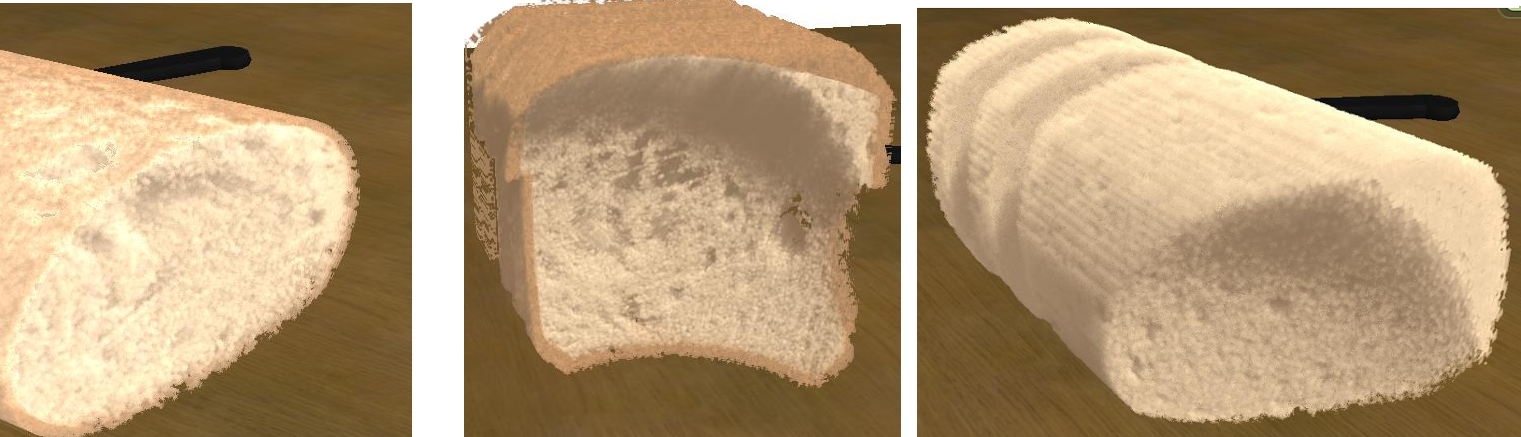
\includegraphics[width=13cm]{fig5}}
  \caption{Imágenes de diferentes tipos de pan renderizados en tiempo real. La imagen de la derecha muestra un pan sin corteza}
  \label{fg:fig5}
\end{figure*}

Es posible obtener otros materiales (ver Fig.~\ref{fg:fig6}). Estos son el resultado de la variación de parámetros técnicos y artísticos del modelo. En las imágenes de prueba pueden distinguirse un budín (izquierda), un pedazo de torta (medio) y una esponja (derecha). En el caso de la esponja se modificaron los parámetros que definen la función de densidad. Cuando no hay levadura en el proceso de creación puede utilizarse una textura volumétrica cuyos valores provienen de una función aleatoria. La retroiluminación es también aproximada con este modelo (ver Fig.\ref{fg:fig7}). En esa imagen puede apreciarse una esponja retroiluminada junto con la propagación de luz a través del volumen que representa.

\begin{figure*}[htb!]
  \centerline{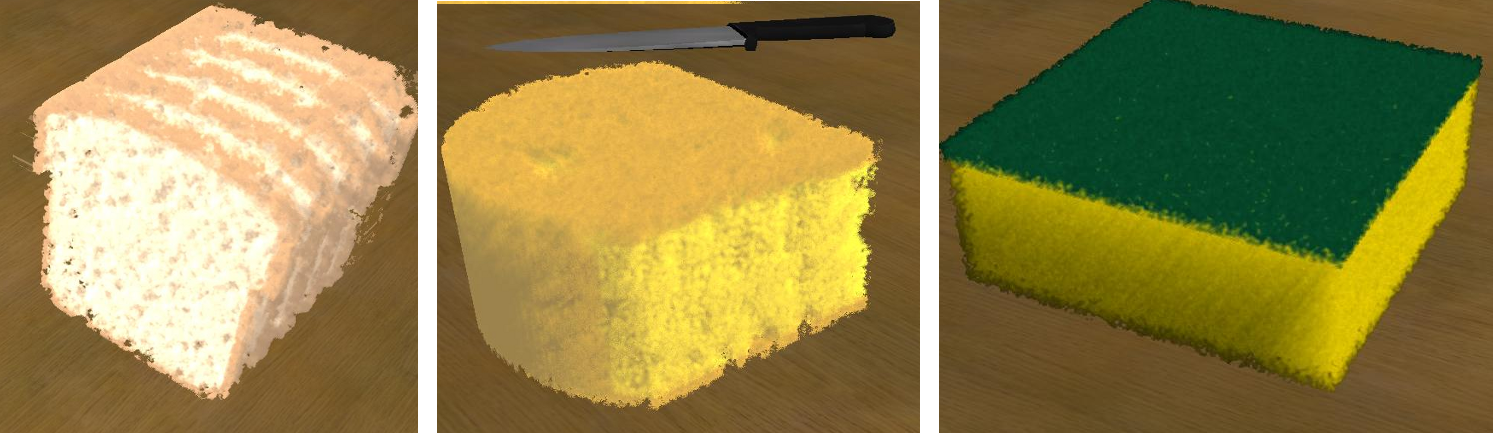
\includegraphics[width=13cm]{fig6}}
  \caption{Distintos materiales obtenidos a partir de diferentes configuraciones de parámetros. De izquierda a derecha: budín, torta y esponja. }
  \label{fg:fig6}

\end{figure*}

\begin{figure*}[htb!]
  \centerline{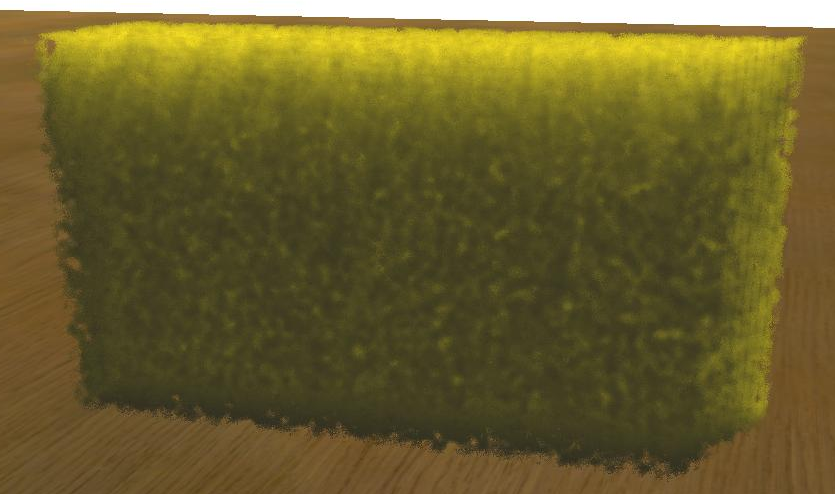
\includegraphics[width=8cm]{fig7}}
  \caption{Esponja retroiluminada.}
  \label{fg:fig7}
\end{figure*}

\subsection{Tiempos de renderizado}

La mayoría de las imágenes se obtuvieron con tasas de refresco de tiempo real (más de 30 FPS), como muestra la Tabla~\ref{tab:n1}. La eficiencia del proceso se resiente cuando la transmitancia es muy baja (el material es casi transparente), dado que se evaluarán más puntos en los rayos a recorrer antes de llegar al límite de transmitancia. Otro parámetro importante es la distancia entre puntos a evaluar. En la Tabla~\ref{tab:n2} se observa que a medida que la cantidad de rayos y de pasos del rayo aumenta, la velocidad decrece. La tabla muestra que los rayos secundarios constituyen el principal cuello de botella, lo cual es lógico, dado que a cada paso del rayo principal, el mismo computa un rayo secundario hacia la luz.

Experimentalmente se encontró que para todos los casos a evaluar $100$ puntos o más presenta buenos resultados.El proceso escala automáticamente con el número de procesadores en una GPU, por lo cual la tasa de refresco obtenida será mayor en GPUs más rápidas y de más procesadores.


ACTUALIZAR!
\begin{table}[htb]
\centering
\begin{tabular}{|c|c|c|c|c|c|c|}
\hline &  Pan 1 & Pan 2 & Pan 3 & Budín & Torta & Esponja \\
\hline
\hline
 FPS promedio  & 32.2 &  75.5 &  45.2 & 28.5 &  54.2 & 29.7\\
\hline
 Puntos de evaluación &  140 &  140 &  140 & 256 &  140 & 256 \\
\hline
 Transmitancia &  15 &  15 &  15 & 15 &  15 & 2.25 \\
\hline
\end{tabular}
\caption{Tiempos de renderizado y parámetros de las imágenes de prueba.}
\label{tab:n1}
\end{table}

\begin{table}[htb]
\centering
\begin{tabular}{|c|c|c|c|c|c|c|}
\hline
 Pasos del rayo         & 128 &  256 \\
\hline
\hline
 Tiempo total shaders   & 10 ms &  32.5 ms \\
\hline
 Rayo Principal         & 2 ms  & 5 ms  \\
\hline
 Rayos Secundarios      &  8 ms & 27.5 ms  \\
\hline
\end{tabular}
\caption{Detalle de tiempos de renderizado en milisegundos.}
\label{tab:n2}
\end{table}


\section{Resultados}
We employed a nVidia GTX 480 ($480$ shader units), which is a typical user configuration.
The CPU is an Intel(R) Core(TM) i5-2300 CPU (quad core).
The screen resolution is $1440\times900$.
In fig.~\ref{fg:application} we show a real-time rendered bread.
Different kinds of bread can be easily modeled changing the parameters of the algorithms (see Fig.~\ref{fg:crumb}).
In Fig.~\ref{fg:results2} we added crust to enhance the final results. 
We also synthesized sponges (see Fig.~\ref{fg:sponges}) with yet different parameter values.
They were easily derived by changing the color and the structure of the volume.
Since yeast is unnecessary in the sponge manufacturing process, we used a random volume texture as a geometry.

We also handled back illumination in the model (see Fig.~\ref{fg:backillum}): the render shows the light propagation in the medium when illuminated from behind.
This is a natural consequence of the RTE based algorithm and the choice of the volume representation that we made.

\subsection*{Computing times}

We rendered all images in real time (FPS over 30). Two parameters are responsible for most of the computations: the transmittance coefficient and the step count.
A low transmittance produces a more transparent material making the ray accumulate more information.

The step count is crucial since for each step we compute the transmittance to the light using a secondary ray.
We experimentally found that values above $140$ give reasonably images for sponges but we needed at least $300$ steps to get a reasonably bread appearance, see Fig.~\ref{fg:stepcount}.
The process automatically scales with the number of GPU processors, so the fps count will increment in more powerful GPUs. 
The use of crust slightly boosts the performance since the transmittance is lower for crust regions, {\em i.e.}, the rays need lower step counts to reach a threshold opacity level.


\section{Otros Materiales Renderizados}

%\section{Conclusiones}

%Según el conocimiento de los autores, éste es el primer intento de llevar a cabo una renderización en tiempo real de pan de manera convincente sin el uso de procesos intermedios complicados (captura de imágenes, generación de mallas, post-procesamiento). Existen buenos resultados de renderizado de pan obtenidos con otros métodos \cite{Cho2007}, pero es difícil comparar ese trabajo con el presentado en este artículo debido a que ni los detalles de la técnica utilizada ni los tiempos de cálculo han sido publicados.

%Dentro del volumen a renderizar se pueden definir regiones con diferentes propiedades. Esta idea permite generar imágenes con miga y corteza con diferentes parámetros.

%La integración de la técnica descrita con motores gráficos es simple. La información de profundidad de los fragmentos puede obtenerse de manera sencilla y por lo tanto pueden utilizarse técnicas populares de sombras, tales como mapas de sombras.

%Los tiempos de cómputo muestran una alta eficiencia del proceso, lo cual depende en gran medida del número de puntos de evaluación usados y la transmitancia del material. Se pueden alcanzcar tiempos de cómputo consistentes con aplicaciones de tiempo real en todos los casos menos en los cuales el volumen ocupa la mayor parte de la imagen a generar, dado que la técnica se calcula casi enteramente en los shader de fragmentos. 

\section*{Discussion}

%1)En primer lugar, un resumen de lo que hicimos en el paper y por qué es importante/novedoso

To the best of the authors' knowledge, this is the first attempt to convincingly render bread crumb and other materials in real time without introducing complex intermediate processes (capture, mesh generation, precomputation, post-process).
There are few previous approaches to bread rendering. An example is \cite{Cho2007}, but comparisons with this technique could not be established since key details are unexplained (computing times, render method).
The proposed method is compatible with current rasterization-based real-time GPU rendering pipelines, providing a realistic looking material, and can be easily integrated into  shader-based 3D engines.
Also, the presented shadow mapping technique allows a natural integration of the volume within scenes. 

%3) Recordamos que las imagenes obtenidas fueron buenas, y que obtuvimos otros materiales cambiando pocos parametros

The modeling and rendering algorithms are flexible enough to model different materials like bread or sponges, changing a few parameters.
Other materials such as cakes, pizzas and cheeses can be implemented in the same way, allowing to manage several materials using the same method.
Also, our volume representation method allows to make real time cuts in the bread crumb.
This is clearly useful in many applications, for instance in video games.

Regarding the illumination model, the success of our algorithms in rendering realistic bread crumbs and other materials could be attributed to the improvements we added to the basic DVR algorithm.
A remarkable improvement in the final realism was due to the addition of an ambient occlusion term, giving the texture a more rich and complex appearance.
Other effects, such as the Phong specular component, enhanced the bread crumb final appearance.
More sophisticated specular methods (for instance, Cook-Torrance model \cite{Cook1982}) did not add a significant improvement.

%5)Tiempos de cómputo (muy importante en este paper!)

Computing times were adequate for real-time rendering in standard off-the-shelf computers (we employed a nVidia GTX 480 GPU with an Intel(R) i5 processor).
Reasonable framerates are always achieved except when the rendered object encompasses a big portion of the screen, since the approach is largely fragment-shader bound.
The final framerate also depends on the step count and the transmittance coefficient.
In addition, different materials require different computing costs for rendering.
For instance, an adequate step count to simulate sponge is lower than the bread crumbs step count.
This can be attributed to the fact that the method needs more steps to capture the macroscopic bread bubbles in crumb.
So far, with current off-the-shelf hardware, our method is limited in the final 3D resolution of the material when real-time applications are required.
In other words, drastic close-ups to the structure could lead to homogeneous areas.
This limitation is tied to the GPU texture size, and will be eventually circumvented with next generations of hardware.
In off-line applications, memory swap procedures allow more satisfactory 3D resolutions.


\section*{Conclusions}

In this paper we applied the transmittance direct volume rendering model using the GPU to a 3D scalar field representing the bread crumb structure, obtaining realistic bread crumb images.
We modeled this structure using particle systems and dynamical systems.
We employed a numerical simulation to solve the resulting set of equations which represents the dynamical system. 
The particles avoided each other and grew following the dynamic system.
The modeling algorithm was easily implemented. 
We implemented the render algorithm in the fragment shader using specular and diffuse components, ambient occlusion and automatic crust determination.

Results showed high fidelity images in real time, suitable for application in several areas, such as video games, serious games \cite{Susi2007} and photorealistic rendering. 
These techniques are much simpler and does not present the drawbacks of other state of the art methods, such as capture processes or mesh generation.
These results make us believe that the volume representation is a right choice for bread modeling and rendering.

As possible continuations of this work, we may extend DVR to handle other phenomena such as indirect illumination, enhancing the resulting images.
Other porous materials such as cheeses will be investigated.
We will employ a number of possible solutions to overcome the resolution problem, such as setting different volume textures depending on the distance between the camera and the volume. 



\begin{figure}
  \centerline{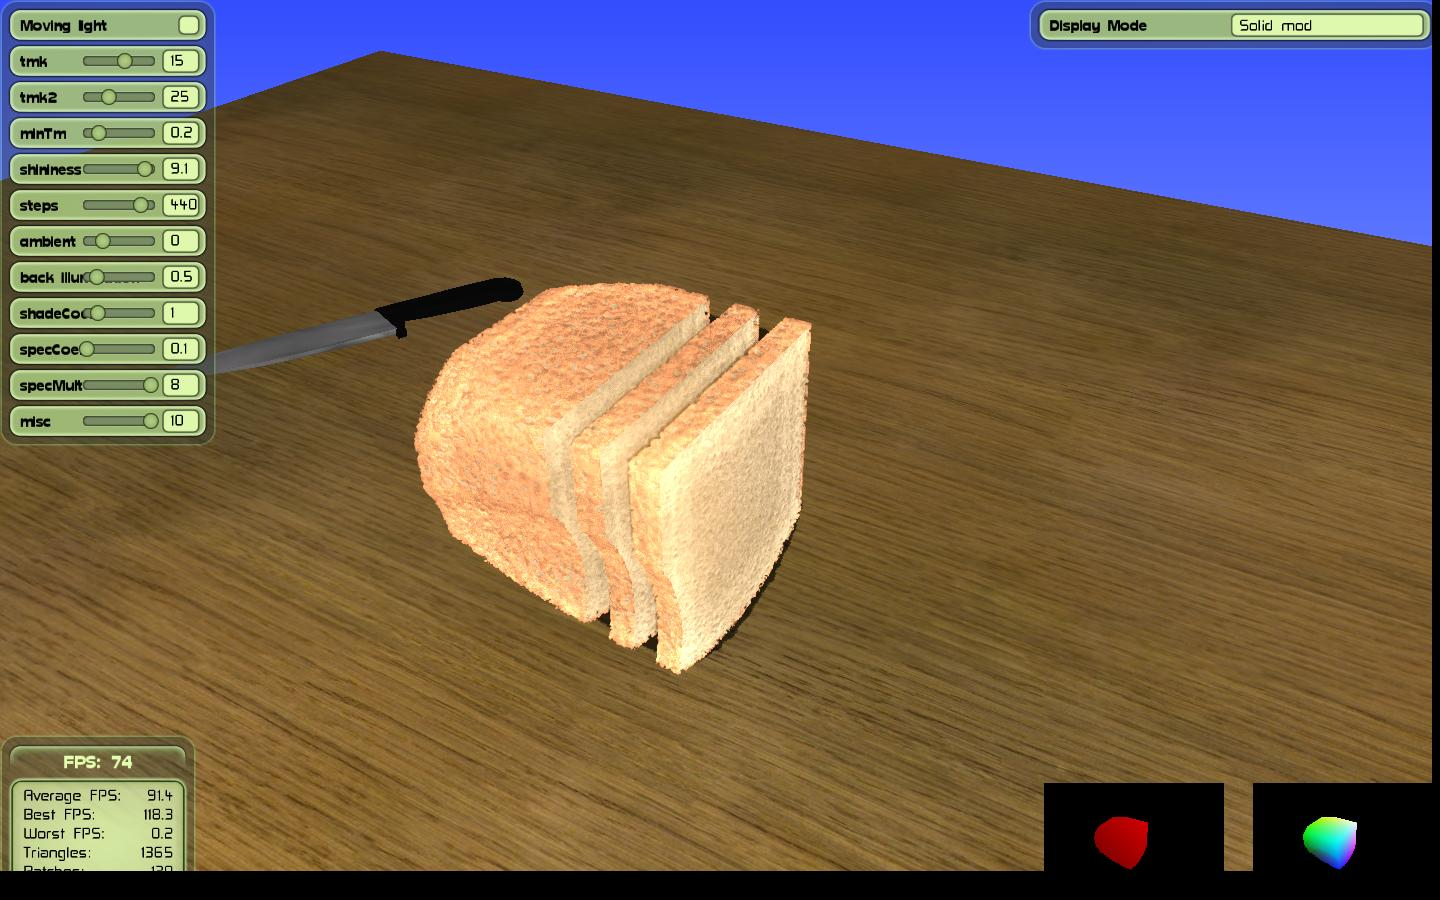
\includegraphics[width=13cm]{figures/application}}
  \caption{Our demo application showing a real time rendered bread.}
  \label{fg:application}
\end{figure}

\begin{figure}
  \centerline{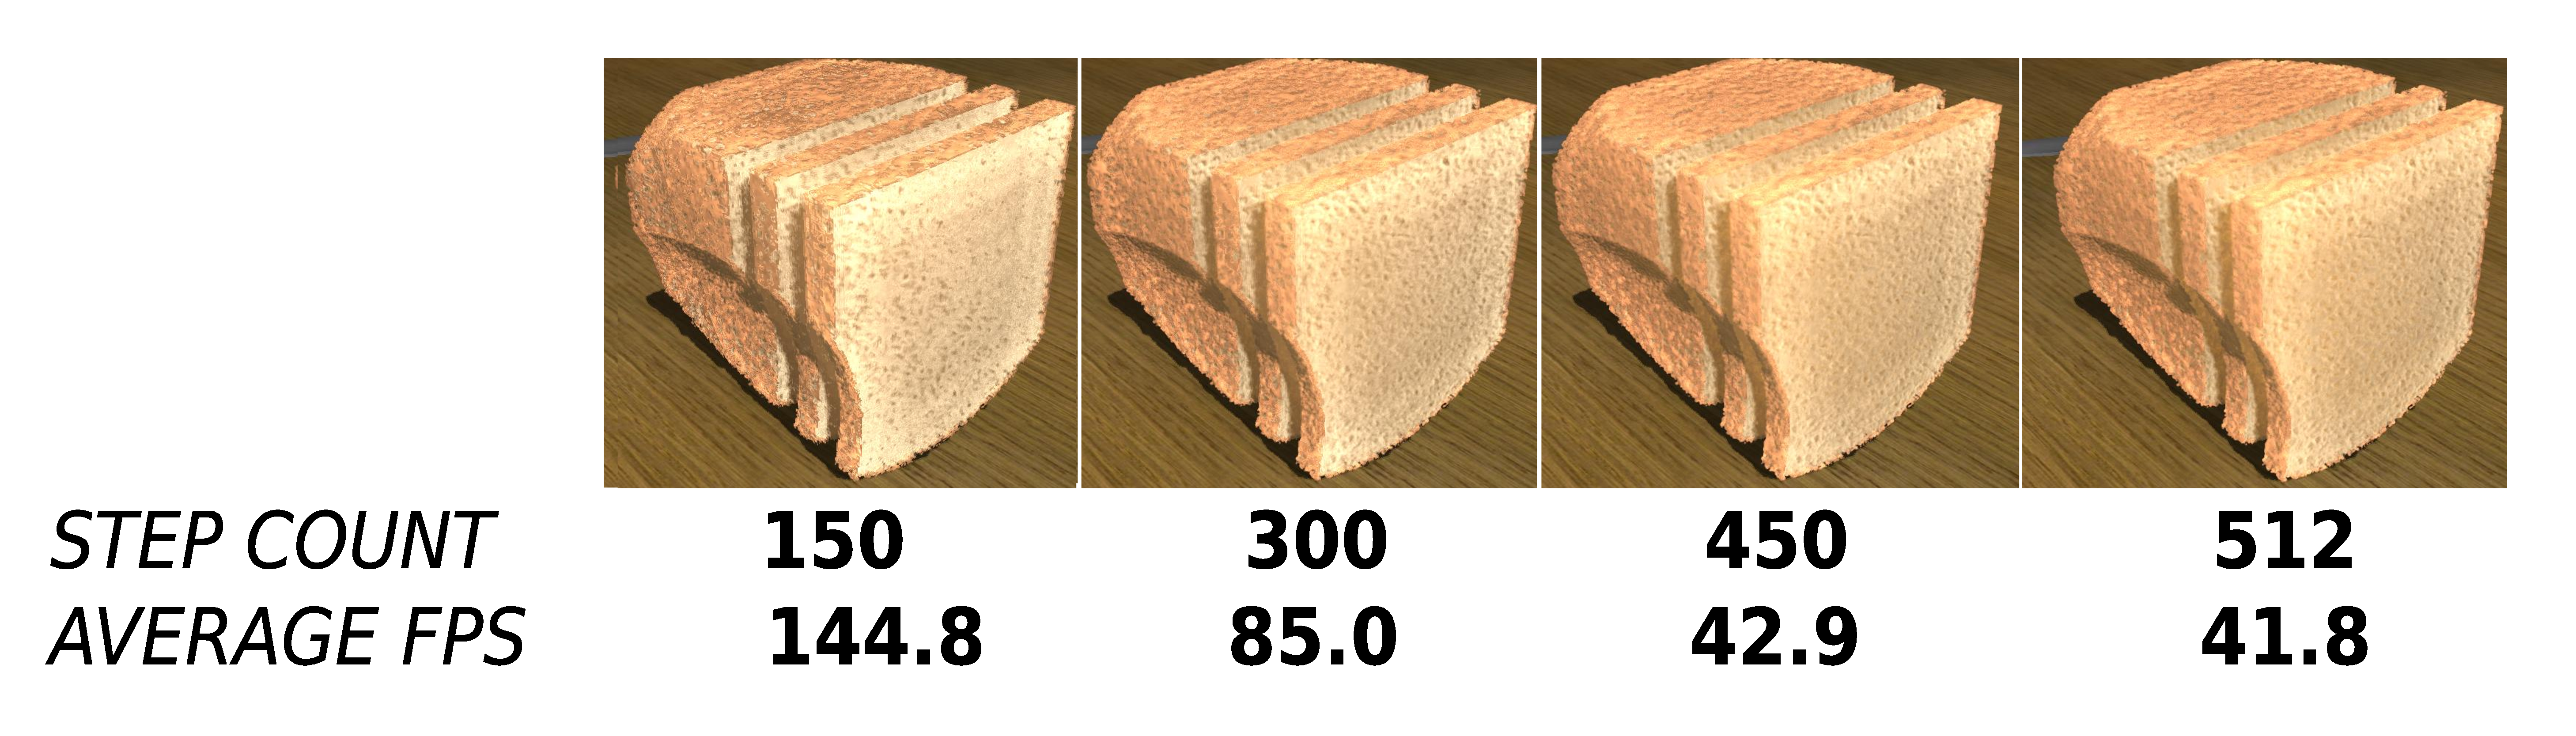
\includegraphics[width=13cm]{figures/stepcount}}
  \caption{Computing times and step count. The image shows that using $300$ sampling ray steps gives reasonably images. }
  \label{fg:stepcount}
\end{figure}

\begin{figure}
  \centerline{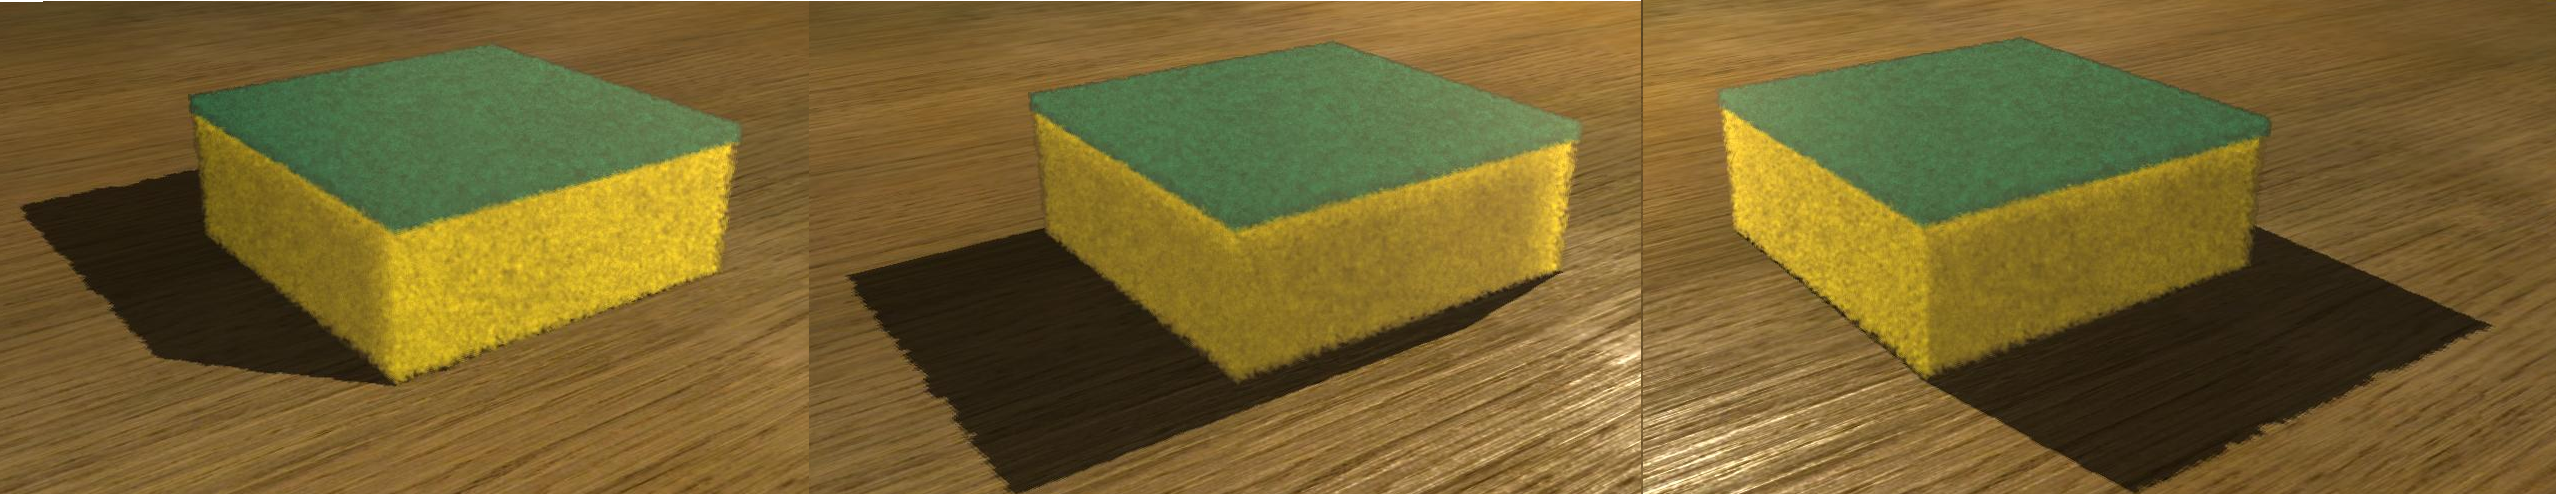
\includegraphics[width=13cm]{figures/sponges}}
  \caption{Real time rendered sponges using a random scalar field as geometry.}
  \label{fg:sponges}
\end{figure}

\begin{figure}
  \centerline{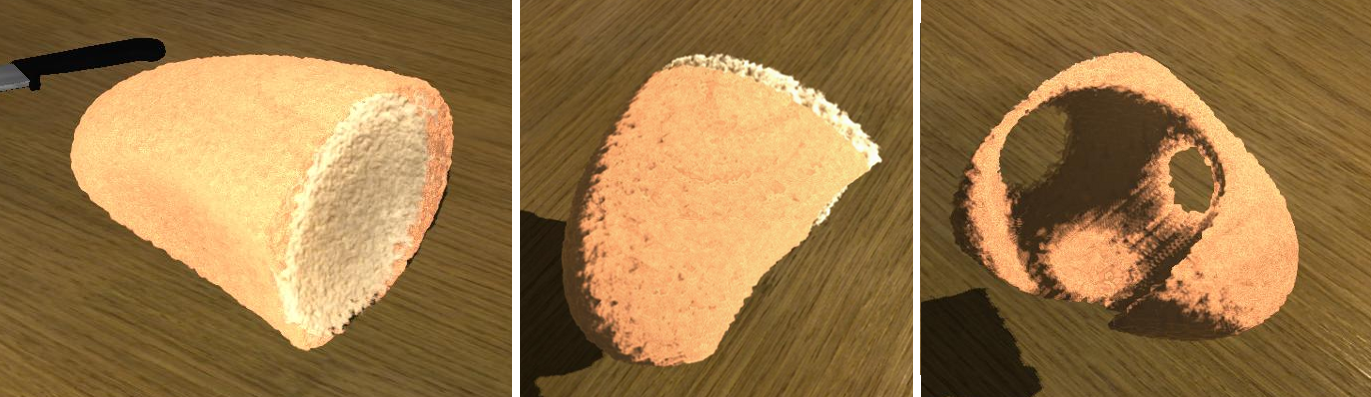
\includegraphics[width=13cm]{figures/crusts}}
  \caption{Crust determination using mathematical morphology. The right image shows that the method works even in extreme cases where the scalar field has holes. }
  \label{fg:crusts}
\end{figure}

\begin{figure}
\centerline{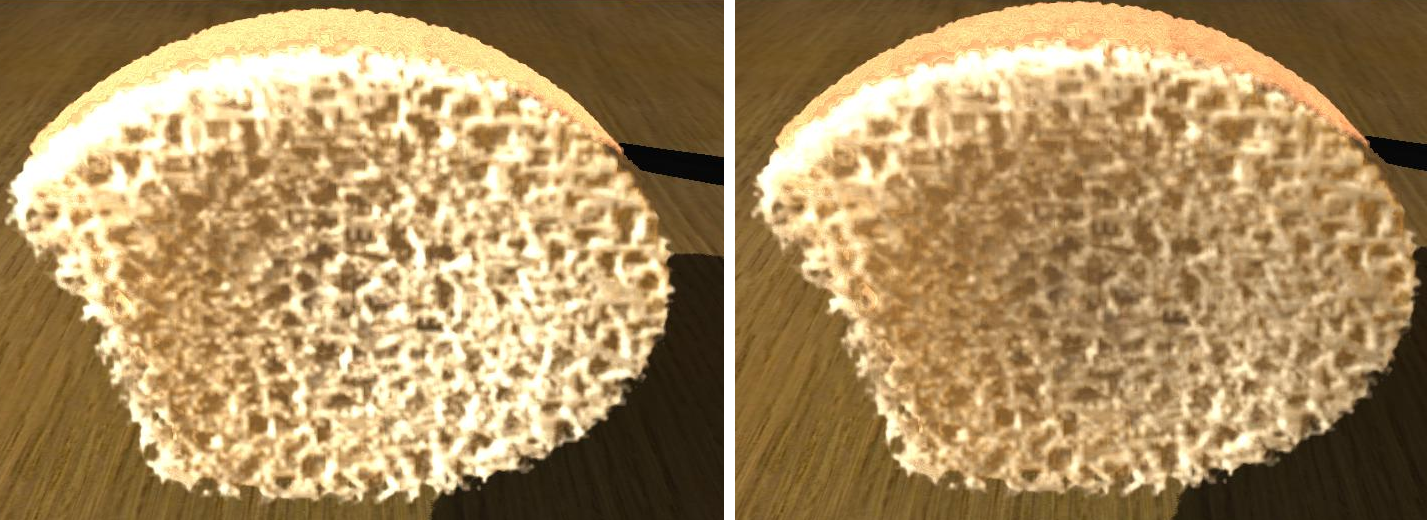
\includegraphics[width=13cm]{figures/occlusion}}
  \caption{Bread without (left) and with (right) ambient occlusion. The final appearance is greatly improved, showing a more natural look. }
  \label{fg:occlusion}
\end{figure}
